% !TEX root = task-1-14-4.tex
% Editable task bank. Append new BankTask blocks at the end of the document.
\documentclass[12pt,a4paper]{article}
\usepackage{physics-textbook}
\usepackage{graphicx,needspace}
\usetikzlibrary{decorations.pathmorphing}
\newif\ifShowSolutions
\ifdefined\TutorEdition
  \ShowSolutionstrue
\else
  \ShowSolutionsfalse % Change to \ShowSolutionstrue to display solutions.
\fi
\newcounter{banktask}
\newsavebox{\BankTaskBox}
\newcommand{\BankTaskContent}[3]{%
  \noindent\textbf{\thebanktask.}\quad #2\par
  \ifShowSolutions
    \Needspace{50mm}% Keep the solution heading with its opening text or diagram.
    #3\par
    \ifdefined\TutorEdition
      \ifcsname TutorSource#1\endcsname
        \nopagebreak\smallskip{\small\csname TutorSource#1\endcsname\par}%
      \fi
    \fi
  \fi
}
\newcommand{\BankTask}[3]{%
  \refstepcounter{banktask}\par\medskip
  \sbox{\BankTaskBox}{\begin{minipage}{\linewidth}%
    \BankTaskContent{#1}{#2}{#3}\end{minipage}}%
  \ifdim\dimexpr\ht\BankTaskBox+\dp\BankTaskBox\relax>\dimexpr\textheight-20mm\relax
    \Needspace{35mm}\BankTaskContent{#1}{#2}{#3}%
  \else
    \Needspace{\dimexpr\ht\BankTaskBox+\dp\BankTaskBox\relax}%
    \noindent\usebox{\BankTaskBox}\par
  \fi
  \medskip
}
\begin{document}
\BookSubsection{1.14.4}{Закон сохранения импульса}


% Source sdamgia-422: https://phys-ege.sdamgia.ru/problem?id=422
\BankTask{sdamgia-422}{
Охотник массой $60\,\text{кг}$, стоящий на гладком льду, стреляет из ружья в горизонтальном направлении. Масса заряда $0{,}03\,\text{кг}$. Скорость дробинок при выстреле $300\,\text{м/с}.$ Какова скорость охотника после выстрела?
}{
\smallskip\noindent\textbf{Решение}\par
Для охотника с ружьем выполняется закон сохранения импульса, поскольку на эту систему не действует никаких внешних сил в горизонтальном направлении: 

$m_{\text{ох}}v_{\text{ох}}=m_{\text{п}}v_{\text{п}}.$

Отсюда находим скорость охотника после выстрела: 

$v_{\text{ох}}=\frac{m_{\text{п}}v_{\text{п}}}{m_{\text{ох}}}=\frac{0{,}03\cdot300}{60}=0{,}15\,\text{м/с}.$

Ответ: $0{,}15$.
}

% Source sdamgia-8934: https://phys-ege.sdamgia.ru/problem?id=8934
\BankTask{sdamgia-8934}{
Тележка движется по инерции по гладким горизонтальным рельсам со скоростью $4\,\text{м/с}$. На тележку вертикально сверху аккуратно опускают мешочек с песком. Масса мешочка в $3$ раза меньше массы тележки. Чему будет равен модуль скорости тележки с мешочком после того, как проскальзывание мешочка относительно тележки прекратится?
}{
\smallskip\noindent\textbf{Решение}\par
Запишем закон сохранения импульса:

$3mV_1=(3m+m)V_2,$

где $m$ — масса мешочка с песком. Найдем отсюда скорость тележки с мешочком:

$V_2=\frac34V_1=3\,\text{м/с}.$

Ответ: $3$.
}

% Source sdamgia-19924: https://phys-ege.sdamgia.ru/problem?id=19924
\BankTask{sdamgia-19924}{
Два шарика массами $m_{1}=0{,}01\,\text{кг}$ и $m_{2}=0{,}02\,\text{кг}$ движутся навстречу друг к другу с одинаковыми скоростями, равными $v=0{,}5\,\text{м/с}$. Найти скорость шариков после абсолютно неупругого столкновения. Округлите до сотых.
}{
\smallskip\noindent\textbf{Решение}\par
Шарики движутся навстречу друг другу. После абсолютно неупругого столкновения они будут двигаться в сторону движения шарика с наибольшим начальным импульсом. Поэтому закон сохранения импульса в проекциях запишется следующим образом: $m_2v-m_1v=u(m_2+m_1).$ Откуда: 

$u=\frac{v(m_2-m_1)}{m_2+m_1}=\frac{0{,}5\cdot0{,}01}{0{,}03}\approx0{,}17\,\text{м/с}.$ 

Ответ: $0{,}17$.
}

% Source sdamgia-2528: https://phys-ege.sdamgia.ru/problem?id=2528
\BankTask{sdamgia-2528}{
Человек массой $50\,\text{кг}$ прыгает с неподвижной тележки массой $100\,\text{кг}$ с горизонтальной скоростью $3\,\text{м/с}$ относительно тележки. Какова скорость тележки относительно Земли после прыжка человека?
}{
\smallskip\noindent\textbf{Решение}\par
Поскольку на систему человек — тележка в горизонтальном направлении не действует никаких сил, для нее в этом направлении выполняется закон сохранения импульса. В системе отсчета, связанной с Землей, в проекции на горизонтальную ось имеем: 

$m_{\text{чел.}}(v_{\text{чел. отн. тел.}}-V_{\text{тел. отн. Зем.}})-M_{\text{тел.}}V_{\text{тел. отн. Зем.}}=0.$

Отсюда находим скорость тележки относительно Земли:

$V_{\text{тел. отн. Зем.}}=\frac{m_{\text{чел.}}v_{\text{чел. отн. тел.}}}{M_{\text{тел.}}+m_{\text{чел.}}}=\frac{50\cdot3}{100+50}=1\,\text{м/с}.$

Ответ: $1$.
}

% Source sdamgia-5357: https://phys-ege.sdamgia.ru/problem?id=5357
\BankTask{sdamgia-5357}{
Мальчик массой $50\,\text{кг}$ находится на тележке массой $50\,\text{кг}$, движущейся по гладкой горизонтальной дороге со скоростью $1\,\text{м/с}$. Каким станет модуль скорости тележки, если мальчик прыгнет с нее со скоростью $2\,\text{м/с}$ относительно дороги в направлении, противоположном первоначальному направлению движения тележки?
}{
\smallskip\noindent\textbf{Решение}\par
Вдоль горизонтальной оси на тележку и мальчика не действуют силы, поэтому по закону сохранения импульса импульс системы вдоль горизонтальной оси сохраняется:

$p_0=p_1+p_2\Longleftrightarrow(M+m)v_0=MV-mv,$

где $M$ — масса тележки, $m$ — масса мальчика, $v_0$ — проекция начальной скорости тележки, $V$ и $v$ — проекции скоростей тележки и мальчика относительно дороги после прыжка мальчика соответственно.

Найдем проекцию скорости тележки $V:$

$V=\frac{(M+m)v_0+mv}{M}=\frac{100\cdot1+50\cdot2}{50}=4\,\text{м/с}.$

Ответ: $4$.
}

% Source sdamgia-5392: https://phys-ege.sdamgia.ru/problem?id=5392
\BankTask{sdamgia-5392}{
Мальчик массой $50\,\text{кг}$ находится на тележке массой $50\,\text{кг}$, движущейся слева направо по гладкой горизонтальной дороге со скоростью $1\,\text{м/с}$. Каким станет модуль скорости тележки, если мальчик прыгнет с нее в направлении первоначальной скорости тележки со скоростью $3\,\text{м/с}$ относительно дороги?
}{
\smallskip\noindent\textbf{Решение}\par
Вдоль горизонтальной оси на тележку и мальчика не действуют силы, поэтому по закону сохранения импульса импульс системы вдоль горизонтальной оси сохраняется:

$p_0=p_1+p_2\Longleftrightarrow(M+m)v_0=mv+MV,$

где $M$ — масса тележки, $m$ — масса мальчика, $v_0$ — проекция начальной скорости тележки, $V$ и $v$ — проекции скоростей тележки и мальчика относительно дороги после прыжка мальчика соответственно.

Найдем проекцию скорости тележки $V$:

$V=\frac{(M+m)v_0-mv}{M}=\frac{100\cdot1-50\cdot3}{50}=-1\,\text{м/с}.$

Знак «минус» означает, что тележка стала двигаться влево. Модуль скорости равен $1\,\text{м/с}$.

Ответ: $1$.
}

% Source sdamgia-24944: https://phys-ege.sdamgia.ru/problem?id=24944
\BankTask{sdamgia-24944}{
Из незакрепленной пушки стреляют снарядом массой $20\,\text{кг}$, который вылетает из ствола в горизонтальном направлении со скоростью $102\,\text{м/с}$ относительно пушки. Пушка при этом откатывается, приобретая относительно земли скорость $2\,\text{м/с}$. Чему равна масса пушки, если массой сгоревшего порохового заряда можно пренебречь?
}{
\smallskip\noindent\textbf{Решение}\par
По закону сохранения импульса $0=m_1\vec v_1+m_2\vec v_2.$ Причем, скорость снаряда относительно земли по правилу сложения скоростей равна $\vec v_1=\vec v_{\text{отн}}+\vec v_2.$ Тогда получаем: $0=m_1(\vec v_{\text{отн}}+\vec v_2)+m_2\vec v_2.$ Учитывая, что пушка откатится в сторону, противоположную направлению движения снаряда, получаем проекцию данного уравнения на горизонтальную ось: $0=m_1v_{\text{отн}}-m_1v_2-m_2v_2,$ откуда получаем искомую величину: 

$m_2=\frac{m_1(v_{\text{отн}}-v_2)}{v_2}=\frac{20\cdot(102-2)}2=1000\,\text{кг}.$

Ответ: $1000$.
}

% Source sdamgia-38976: https://phys-ege.sdamgia.ru/problem?id=38976
\BankTask{sdamgia-38976}{
На краю стола высотой $h=1{,}25\,\text{м}$ лежит пластилиновый шарик массой $m=50\,\text{г}$. На него со стороны стола налетает по горизонтали другой пластилиновый шарик, имеющий скорость $v=1\,\text{м/с}.$ Какой должна быть масса второго шарика, чтобы точка приземления шариков на пол была дальше от стола, чем заданное расстояние $L=0{,}4\,\text{м}$? Удар считать центральным.
}{
\smallskip\noindent\textbf{Решение}\par
Обоснование
Систему отсчета, связанную с Землей, будем считать инерциальной. Тела движутся поступательно, поэтому их можно принять за материальные точки. По условию задачи силой сопротивления воздуха можно пренебречь. Поэтому тела движутся в поле Земного тяготения. Следовательно, для описания движения тел после столкновения можно использовать законы равноускоренного движения.
Перед столкновением на шарики действуют силы тяжести, которые являются внешними. Поскольку при столкновении на шарики действуют внутренние силы взаимодействия, которые довольно велики из-за кратковременности удара, то по сравнению с ними силой тяжести можно пренебречь, а значит можно пренебречь внешними силами, действующими на тела в процессе соударения. Поэтому можно воспользоваться законом сохранения импульса.

Перейдем к решению. Так как соударение неупругое, то после него шарики будут двигаться как одно целое. Запишем закон сохранения импульсов тел при неупругом ударе: $Mv=(m+M)u,$ где $M$ — масса движущегося шарика, $u$ — скорость шариков после неупругого соударения.
После соударения скорость шариков будет направлена горизонтально. Они будут двигаться с ускорением свободного падения, направленного вниз. Движение по оси $Ox$ будет равномерным, так как $g_x=0,$ поэтому дальность полета шариков равна $L=u_xt,$ где $t$ — время полета шариков о пол, причем $u_x=u.$
Движение по оси $Oy$ — равноускоренное с ускорением $g_y=g$ и проекцией начальной скорости $u_y=0.$ Поэтому высота, с которой брошены шарики $h=\frac{gt^2}2.$
Тогда время полета шариков $t=\sqrt{\frac{2h}g},$ дальность полета $L=u\sqrt{\frac{2h}g}.$ Скорость шариков после соударения:

$u=L\sqrt{\frac g{2h}}=0{,}4\sqrt{\frac{10}{2\cdot1{,}25}}=0{,}8\,\text{м/с}.$

Тогда находим массу второго шарика:

$M=\frac{mL\sqrt{g/(2h)}}{v-L\sqrt{g/(2h)}}$

Точка приземления шариков будет больше $L$, если масса второго шарика будет 

$M>\frac{mL\sqrt{g/(2h)}}{v-L\sqrt{g/(2h)}}=\frac{0{,}05\cdot0{,}8}{1-0{,}8}=0{,}2\,\text{кг}=200\,\text{г}.$

Ответ: $M>200\,\text{г}.$
}

% Source sdamgia-43208: https://phys-ege.sdamgia.ru/problem?id=43208
\BankTask{sdamgia-43208}{
При разрыве снаряда суммарная энергия системы увеличивается за счет энергии взрыва. На сколько изменится суммарная энергия системы, если снаряд массой $M=9\,\text{кг}$, летящий со скоростью $250\,\text{м/с}$, разорвется на две части: первая продолжит движение по направлению движения снаряда со скоростью $900\,\text{м/с}$, а вторая — в обратном направлении? Считать, что масса первой и второй части снаряда равны $\frac M3$ и $\frac{2M}3$ соответственно. Обоснуйте применение физических законов, использованных при решении задачи.
}{
\smallskip\noindent\textbf{Решение}\par
Обоснование. 
$1$. Данную задачу рассмотрим в системе отсчета, связанную с Землей, которую в этих условиях можно считать инерциальной. 
$2$. Снаряд и его части движутся поступательно, поэтому их можно описывать моделью материальной точки.
$3$. Для материальных точек в инерциальной системе отсчета за малый промежуток времени применим закон сохранения импульса.
$4$. За малый промежуток взаимодействия частей снаряда можно считать, что потенциальная энергия тел не изменилась.

Перейдем к решению.
Запишем закон сохранения импульса:

$M\vec v=\frac M3\vec u_1+\frac{2M}3\vec u_2,$
$Ox$: $3v=u_1-2u_2,$

где $u_{2}$ − скорость второго осколка после взрыва, которая равна 

$u_2=\frac{u_1-3v}2=\frac{900-3\cdot250}2=75\,\text{м/с}.$

По закону изменения кинетической энергии $\Delta E=E_2-E_1,$ где начальное и конечное значения кинетической энергии:

$E_1=\frac{Mv^2}2;$ $E_2=\frac{Mu_1^2}{2\cdot3}+\frac{2Mu_2^2}{2\cdot3}$
$\Delta E=\frac M2\left(\frac{u_1^2+2u_2^2}3-v^2\right)=\frac92\left(\frac{900^2+2\cdot75^2}3-250^2\right)=950625\,\text{Дж}.$

Ответ: $950625\,\text{Дж}$.
}

% Source sdamgia-25948: https://phys-ege.sdamgia.ru/problem?id=25948
\BankTask{sdamgia-25948}{
На двух невесомых нерастяжимых вертикальных нитях подвешена горизонтальная пробирка с газом, закрытая пробкой. Масса пробирки $M=0{,}05\,\text{кг}$, длина нитей $L=0{,}4\,\text{м}$, нить рвется, когда к ней прикладывается сила $T=0{,}5\,\text{Н}$. При нагревании подвешенной пробирки из нее вылетает пробка массой $m$ со скоростью $10\,\text{м/с}$. Найти минимальную массу пробки, при которой в момент ее вылета нити разорвутся.
Какие законы Вы используете для описания взаимодействия пробирки и пробки? Обоснуйте их применение к данному случаю.
}{
\smallskip\noindent\textbf{Решение}\par
Обоснование
Систему отсчета, связанную с Землей, будем считать инерциальной. Силы сопротивления воздуха не оказывают влияние на движение пробки и пробирки, поскольку они пренебрежимо малы. Внешние силы реакции опоры и силы тяжести не оказывают действия в горизонтальном направлении (так как сумма их проекций на горизонтальную ось равна нулю). Следовательно, в инерциальной системе отсчета применим закон сохранения импульса.
В нижней точке пробирку можно считать материальной точку, на которую действуют сила натяжения нити и сила тяжести. В инерциальной системе отсчета можно применить второй закон Ньютона. Равнодействующая сил в этой точке является причиной центростремительного ускорения. Значит, можно применять законы равномерного движения тела по окружности.

Перейдем к решению.
$1$. При взаимодействии пробки с пробиркой они приобретут скорости, равные соответственно $v$ и $u$. По закону сохранения импульса $mv=Mu$, откуда $m=\frac{Mu}v.$
$2$. Пробирка приобретет скорость и в нижней точке по второму закону Ньютона $2T-Mg=Ma$. При этом центростремительное ускорение пробирки равно $a=\frac{u^2}L.$ 
Отсюда:

$u=\sqrt{\frac{L(2T-Mg)}M}.$

$3$. Находим искомую массу пробки:

$m=\frac1v\sqrt{ML(2T-Mg)}=\frac1{10}\sqrt{0{,}05\cdot0{,}4\cdot(2\cdot0{,}5-0{,}05\cdot10)}=0{,}01\,\text{кг}=10\,\text{г}.$

Ответ: $10\,\text{г}$.
}

% Source sdamgia-29762: https://phys-ege.sdamgia.ru/problem?id=29762
\BankTask{sdamgia-29762}{
По гладкой наклонной плоскости, составляющей угол $\alpha=30^\circ$ с горизонтом, скользит из состояния покоя брусок массой $M=250\,\text{г}$. В тот момент, когда брусок прошел по наклонной плоскости расстояние $x=3{,}6\,\text{м}$, в него попала и застряла в нем летящая навстречу ему вдоль наклонной плоскости пуля массой $m.$ Скорость пули $v=555\,\text{м/с}$. После попадания пули брусок поднялся вверх вдоль наклонной плоскости на расстояние $S=2{,}5\,\text{м}$ от места удара. Найдите массу пули $m$. Трение бруска о плоскость не учитывать. Обоснуйте применимость используемых законов к решению задачи.
}{
\smallskip\noindent\textbf{Решение}\par
Обоснование
Систему отсчета, связанную с Землей, будем считать инерциальной. В ИСО изменение механической энергии тела равно работе всех приложенных к телу непотенциальных сил. При движении бруска вниз и вверх по наклонной плоскости на него действуют потенциальная сила тяжести и сила реакции опоры $\vec N,$ перпендикулярная перемещению бруска (трения нет, так как поверхность гладкая). Поэтому работа силы $\vec N$ при движении бруска по наклонной плоскости равна нулю. Следовательно, механическая энергия бруска при его движении до удара сохраняется. Аналогично сохраняется механическая энергия бруска и при его движении после удара.
Закон сохранения импульса выполняется в ИСО в проекциях на выбранную ось, если сумма проекций внешних сил на эту ось равна нулю. В данном случае выбранную ось направим параллельно движению бруска. Проекции на эту наклонную ось сил тяжести, действующих на брусок и на пулю, не равны нулю. Но надо учесть, что при столкновении бруска и пули импульс каждого из двух тел меняется на конечную величину, тогда как время столкновения мало. Следовательно, на каждое из двух тел в это время действовала огромная сила (это сила взаимодействия бруска и пули), по сравнению с которой сила тяжести ничтожна. Поэтому при столкновении тел силы тяжести не учитываются. Вследствие этого при описании столкновения бруска с пулей соблюдается закон сохранения импульса для системы тел «брусок + пуля».

Перейдем к решению. 
$1$. Рассмотрим два состояния при движении бруска — в начальный момент времени и в момент попадания пули, который примем на нулевой уровень высоты. В первом состоянии брусок обладал потенциальной энергией $E_{p1}=Mgh_1,$ причем по рисунку $h_1=x\sin\alpha.$ Во втором состоянии брусок обладал кинетической энергией $E_{k2}=\frac{Mv_1^2}2.$ По закону сохранения энергии:

$Mgx\sin\alpha=\frac{Mv_1^2}2.$ 


\begin{center}\begin{tikzpicture}[task graph]
\draw[task curve] (0,0)--(4.5,0)--(4.5,2)--cycle;\draw[task curve] (.6,0) arc (0:24:.6) node[right] {$\alpha$};
\foreach \x in {0,.2,...,4.5}{\draw (\x,0)--++(-.12,-.12);}
\begin{scope}[rotate=24]\draw[fill=orange!25] (2.8,0) rectangle (3.1,.35);\end{scope}\draw[fill=orange!25] (1.5,.8) circle (.1);\draw[task curve,->] (1.6,.84)--(2.2,1.1) node[below left=2pt] {$\vec v_2$};\draw[task curve,->] (2.7,1.25)--(2.1,.98) node[above] {$\vec v_1$};\draw[task curve,<->] (3,1.7)--(4.3,2.28) node[midway,above] {$x$};\draw[task curve] (3,1.3)--(4.5,1.3);\draw[task curve] (4.5,1.3)--(4.5,2) node[midway,right] {$h_1$};
\end{tikzpicture}\end{center}



\begin{center}\begin{tikzpicture}[task graph]
\draw[task curve] (0,0)--(4.5,0)--(4.5,2)--cycle;\draw[task curve] (.6,0) arc (0:24:.6) node[right] {$\alpha$};
\foreach \x in {0,.2,...,4.5}{\draw (\x,0)--++(-.12,-.12);}
\begin{scope}[rotate=24]\draw[fill=orange!25] (2.8,0) rectangle (3.1,.35);\end{scope}\begin{scope}[rotate=24]\draw[fill=orange!25] (1.3,0) rectangle (1.6,.35);\draw[fill=orange!25] (1.38,.13) circle (.08);\end{scope}\draw[task curve,->] (1.4,.9)--(2.1,1.2) node[above] {$\vec v$};\draw[task curve,<->] (1.3,1.3)--(2.9,2.01) node[midway,above] {$S$};\draw[task curve] (1.5,.7)--(2.9,.7)--(2.9,1.3) node[midway,right] {$h_2$};\draw[task curve,<->] (3.1,2.1)--(4.3,2.63) node[midway,above] {$x$};
\end{tikzpicture}\end{center}


$2$. В результате неупругого взаимодействия бруска и пули они станут одним целым и будут двигаться со скоростью $u$ в направлении движения пули. По закону сохранения импульса $m\vec v_2+M\vec v_1=(m+M)\vec u.$ В проекции на ось $Ox$, направленную вверх вдоль наклонной плоскости, получаем $mv_2-Mv_1=(m+M)u.$
$3$. Рассмотрим два состояния бруска с пулей — в момент удара, который будем считать нулевым уровнем высоты, и в момент остановки при подъеме на некоторую высоту $h_2=s\sin\alpha.$ В первом состоянии тела обладают кинетической энергией $E_{k1}=\frac{(M+m)u^2}2,$ во втором состоянии $-$ потенциальной энергией $E_{p2}=(M+m)gh_2.$ По закону сохранения энергии:

$\frac{(M+m)u^2}2=(M+m)gh_2.$ 

$4$. Объединяя записанные уравнения, находим массу пули:

$m=\frac{M(v_1+u)}{v_2-u}=\frac{M(\sqrt{2gx\sin\alpha}+\sqrt{2gs\sin\alpha})}{v_2-\sqrt{2gs\sin\alpha}},$

 то есть:

$m=\frac{250\cdot(\sqrt{2\cdot10\cdot3{,}6\cdot0{,}5}+\sqrt{2\cdot10\cdot2{,}5\cdot0{,}5})}{555-\sqrt{2\cdot10\cdot2{,}5\cdot0{,}5}}=5\,\text{г}.$

Ответ: $5\,\text{г}$.
}

% Source sdamgia-29765: https://phys-ege.sdamgia.ru/problem?id=29765
\BankTask{sdamgia-29765}{
В маленький шар массой $M=250\,\text{г}$, висящий на нити длиной $l=50\,\text{см}$, попадает и застревает в нем горизонтально летящая пуля массой $m=10\,\text{г}$. При какой минимальной скорости пули шар после этого совершит полный оборот в вертикальной плоскости? Сопротивлением воздуха пренебречь. Обоснуйте применимость используемых законов к решению задачи.
}{
\smallskip\noindent\textbf{Решение}\par
\begin{center}\begin{tikzpicture}[task graph]
\draw[fill=orange!25] (0,0) rectangle (.4,.25) node[below] {$m$};\draw[task curve,->] (.4,.15)--(1,.15) node[above] {$\vec v$};\draw[fill=orange!25] (1.6,.15) circle (.2) node[below=6pt] {$M$};
\end{tikzpicture}\end{center}

Обоснование
$1$. Систему отсчета, связанную с Землей, будем считать инерциальной.
$2$. Тела считаем материальными точками.
$3$. Для описания взаимодействия пули и шара использован закон сохранения импульса системы тел. Он выполняется в инерциальной системе отсчета, если сумма внешних сил, приложенных к телам системы, равна нулю. В данном случае проекции внешних сил (силы тяжести и силы натяжения нити) на горизонтальную ось в момент взаимодействия равны нулю. Следовательно, можно использовать закон сохранения импульса в проекциях на эту ось.
$4$. Для дальнейшего движения шара с застрявшей в нем пулей будет справедлив закон сохранения механической энергии, поскольку сопротивлением воздуха по условию задачи можно пренебречь, а единственная неконсервативная сила, действующая на шар, — сила натяжения нити — не совершает работы при движении шара по окружности, поскольку она всюду перпендикулярна скорости движения шара.
$5$. Условие минимальности $v_0$ означает, что шар совершает полный оборот в вертикальной плоскости, но при этом натяжение нити в верхней точке (и только в ней!) обращается в нуль.
\begin{center}\begin{tikzpicture}[task graph]
\draw[task curve] (0,0) circle (1);\draw[task curve] (0,-1)--(0,1);
\draw[fill=orange!25] (0,1) circle (.13);\draw[fill=orange!25] (0,-1) circle (.13);
\draw[task curve,->] (0,1)--(-.9,1) node[above] {$\vec V$};\draw[task curve,->] (0,-1)--(.9,-1) node[below] {$\vec u$};
\draw[task curve,->] (0,1)--(0,.3) node[right] {$(m+M)\vec g$};\draw[task curve,->] (-.25,.7)--(-.25,.1) node[left] {$\vec a$};
\end{tikzpicture}\end{center}


Перейдем к решению.
$1$. Запишем закон сохранения импульса при взаимодействии пули и шарика, учтем, что до взаимодействия шарик покоился, а удар был абсолютно неупругий, $mv=(M+m)u.$ 
$2$. Выберем за начальный уровень высоты нижнюю точку траектории движения шарика с пулей. В этой точке тела обладали кинетической энергией:

$E_{k1}=\frac{(M+m)u^2}2.$

В верхней точке траектории тела обладали потенциальной энергией $E_{p2}=(M+m)gh,$ причем $h=2R,$ и кинетической энергией:

$E_{k2}=\frac{(M+m)V^2}2.$

По закону сохранения энергии:

$\frac{(M+m)u^2}2=\frac{(M+m)V^2}2+(M+m)gh.$ 

$3$. В верхней точке траектории на тела действует сила тяжести, движение с центростремительным ускорением $a=\frac{V^2}R.$ По второму закону Ньютона $(M+m)a=(M+m)g.$ При этом радиус окружности равен длине нити. 
$4$. Объединяя все уравнения, находим скорость пули до взаимодействия:

$v=\frac{M+m}{m}\sqrt{5gR}=\frac{250+10}{10}\sqrt{5\cdot10\cdot0{,}5}=130\,\text{м/с}.$

Ответ: $130\,\text{м/с}$.
}


% Source DC8C1F: https://ege.fipi.ru/bank/questions.php?search=1&proj=BA1F39653304A5B041B656915DC36B38&qid=DC8C1F
\BankTask{DC8C1F}{
Два тела движутся по взаимно перпендикулярным пересекающимся прямым, как показано на рисунке. Модуль импульса первого тела $p_1=8\,\text{кг}\cdot\text{м}/\text{с}$, второго тела $p_2=6\,\text{кг}\cdot\text{м}/\text{с}$. Каков модуль импульса системы этих тел после их абсолютно неупругого удара? Выразите ответ в $\text{кг}\cdot\text{м}/\text{с}$.
\begin{center}
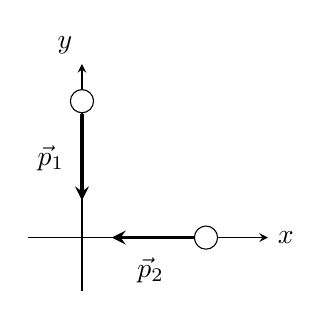
\begin{tikzpicture}[>=stealth,scale=1.05]
\draw[->] (-0.65,0)--(2.25,0) node[right] {$x$};
\draw[->] (0,-0.65)--(0,2.1) node[above left] {$y$};
\draw[fill=white] (0,1.65) circle (0.14);
\draw[very thick,->] (0,1.49)--(0,0.45);
\node[left] at (-0.1,0.96) {$\vec p_1$};
\draw[fill=white] (1.5,0) circle (0.14);
\draw[very thick,->] (1.35,0)--(0.36,0);
\node[below] at (0.83,-0.12) {$\vec p_2$};
\end{tikzpicture}
\end{center}
}{
\smallskip\noindent\textbf{Решение от GPT}\par
Импульс системы сохраняется. До удара импульсы перпендикулярны, поэтому $p=\sqrt{p_1^2+p_2^2}=\sqrt{8^2+6^2}=10\,\text{кг}\cdot\text{м}/\text{с}$. Ответ: $10\,\text{кг}\cdot\text{м}/\text{с}$.
}

% Source 8CED26: https://ege.fipi.ru/bank/questions.php?search=1&proj=BA1F39653304A5B041B656915DC36B38&qid=8CED26
\BankTask{8CED26}{
Сталкиваются и слипаются два разных по массе пластилиновых шарика, причём векторы их скоростей непосредственно перед столкновением направлены навстречу друг другу и одинаковы по модулю: $\upsilon_{1}=\upsilon_{2}=1\,\text{м}/\text{с}$. Во сколько раз масса тяжёлого шарика больше, чем лёгкого, если сразу после столкновения их скорость стала равной (по модулю) $0{,}5\,\text{м}/\text{с}$?
}{
\smallskip\noindent\textbf{Решение от GPT}\par
Положительное направление выберем по движению тяжёлого шарика. По сохранению импульса $(M-m)\cdot1=(M+m)\cdot0{,}5$. Отсюда $M/m=3$.
}

% Source 1D0119: https://ege.fipi.ru/bank/questions.php?search=1&proj=BA1F39653304A5B041B656915DC36B38&qid=1D0119
\BankTask{1D0119}{
Шайба массой $m$, скользящая по гладкой горизонтальной поверхности со скоростью $v$, абсолютно неупруго сталкивается с покоящейся шайбой массой $M$.
\TaskMatchingColumns[.53\linewidth]{Физические величины}{
А) кинетическая энергия покоившейся шайбы после столкновения\par
Б) импульс налетающей шайбы после столкновения
}{Формулы}{
1) $\frac{m^2v}{m+M}$\par
2) $mv$\par
3) $\frac{m^2Mv^2}{2(m+M)^2}$\par
4) $\frac{Mv^2}{2}$\par
}\begin{center}\begin{tabular}{|c|c|}\hline А & Б \\\hline\rule{0pt}{1.2em}\hspace{1cm} & \hspace{1cm} \\\hline\end{tabular}\end{center}
}{
\smallskip\noindent\textbf{Решение от GPT}\par
Из сохранения импульса общая скорость $u=mv/(m+M)$. Энергия второй шайбы $Mu^2/2=m^2Mv^2/[2(m+M)^2]$ (формула $3$); импульс первой $mu=m^2v/(m+M)$ (формула $1$). Ответ: $31$.
}

% Source 48533: https://phys-ege.sdamgia.ru/problem?id=48533
\BankTask{48533}{
Тележка массой $200\,\text{кг}$ покоится на земле. В нее запрыгивает мальчик массой $50\,\text{кг}$ со скоростью $4\,\text{м/с}$. Найдите скорость их движения после взаимодействия.
}{
\smallskip\noindent\textbf{Решение}\par
Движение тел поступательное, поэтому тела можно описывать моделью материальной точки. Система отсчета связана с Землей, которую может считать инерциальной системой отсчета. Время взаимодействия мальчика и тележки мало, действием силы трения можно пренебречь. Следовательно, можем применить закон сохранения импульсов тел.
По закону сохранения импульса тел при неупругом взаимодействии $m_1 v = ( m_1 + m_2 ) u,$ откуда находим скорость движения после взаимодействия:

\[u = \frac{m_1 v}{m_1 + m_2} = \frac{50 \cdot 4}{200 + 50} = 0{,}8 \,\text{м/с}.\]

Ответ: $0{,}8\,\text{м/с}$.
}

% Source 43099: https://phys-ege.sdamgia.ru/problem?id=43099
\BankTask{43099}{
Мальчик массой $50\,\text{кг}$ находится на тележке массой $50\,\text{кг}$, движущейся по гладкой горизонтальной дороге со скоростью $1\,\text{м/с}$. Каким станет модуль скорости тележки, если мальчик прыгнет с нее со скоростью $2\,\text{м/с}$ относительно дороги в направлении, противоположном первоначальному направлению движения тележки? Ответ запишите в метрах за секунду.
}{
\smallskip\noindent\textbf{Решение}\par
Вдоль горизонтальной оси на тележку и мальчика не действуют силы, поэтому по закону сохранения импульса импульс системы вдоль горизонтальной оси сохраняется:

\[p_0=p_1 + p_2 \Longleftrightarrow ( M + m ) v _0=MV - m v ,\]

где M  — масса тележки, m  — масса мальчика, $v _0$  — проекция начальной скорости тележки, V и $v$  — проекции скоростей тележки и мальчика относительно дороги после прыжка мальчика соответственно.

Найдем проекцию скорости тележки $V:$

\[V= \frac{( M + m ) v _0 + m v}{M} \Longleftrightarrow V= \frac{100\,\text{кг} \cdot 1\,\text{м/с} + 50\,\text{кг} \cdot 2\,\text{м/с}}{50\,\text{кг}} =4\,\text{м/с} .\]

Ответ:  $4\,\text{м/с}$.
}

% Source 25942: https://phys-ege.sdamgia.ru/problem?id=25942
\BankTask{25942}{
Небольшое тело массой $M$  =  $0{,}99\,\text{кг}$ лежит на вершине гладкой полусферы. В тело попадает пуля массой $m$  =  $0{,}01\,\text{кг}$, летящая горизонтально со скоростью $\upsilon_{0}$  =  $100\,\text{м/с}$, и застревает в нем. Пренебрегая смещением тела за время удара, определите радиус сферы, если высота, на которой тело оторвется от поверхности полусферы, $h$  =  $0{,}7\,\text{м}$. Высота отсчитывается от основания полусферы.
Какие законы Вы используете для описания взаимодействия тел? Обоснуйте их применение к данному случаю.
}{
\smallskip\noindent\textbf{Решение}\par
Обоснование 
Систему отсчета, связанную с Землей, будем считать инерциальной. Тела можно считать материальными точками, так как их размеры пренебрежимо малы в условии задачи. При соударении для системы «пуля  — тело» в ИСО выполняется закон сохранения импульса в проекции на горизонтальную ось, так как внешние силы (сила тяжести и сила реакции опоры) вертикальны.
При движении составного тела от вершины полусферы выполняется сохранение механической энергии, так как полусфера гладкая, и работа силы реакции опоры равна нулю (эта сила перпендикулярно скорости тела).
В момент отрыва обращается в ноль сила реакции опоры $\vec N.$
Второй закон Ньютона выполняется в ИСО для модели материальной точки.

Перейдем к решению.
$1$.  Запишем закон сохранения импульса в проекции на горизонтальную ось для столкновения пули и тела:

\[m v _0= ( M + m ) V_0.\]

Таким образом, тело с пулей начинают соскальзывать с начальной скоростью:

\[V_0= \frac{m v _0}{M + m} .\]

$2$.  Запишем закон сохранения энергии, чтобы найти скорость тела на высоте $h$ от Земли:

$\frac{( M + m ) V_0 ^2}{2} + ( M + m ) gR= \frac{( M + m ) V ^2}{2} + ( M + m ) gh,$
$V ^2 =V_0 ^2 + 2g ( R - h ) = ( \frac{m v _0}{M + m} ) ^2 + 2g ( R - h ) .$

$3$.  При движении тела по полусфере на него действуют сила тяжести и сила реакции опоры N.
В проекции на нормаль к поверхности полусферы второй закон Ньютона имеет вид:

\[( M + m ) a_{\,\text{ц}}= ( M + m ) \frac{V ^2}{R} = ( M + m ) g \cos \alpha - N.\]

Тело оторвется от поверхности в момент, когда сила реакции опоры будет равна нулю, при этом $\cos \alpha = \frac{h}{R} .$
Выражаем отсюда квадрат скорости тела:

\[V ^2 =gh.\]

$4$.  Подставим это значение в полученное ранее уравнение и найдем радиус полусферы:

$gh= ( \frac{m v _0}{M + m} ) ^2 + 2g ( R - h ) ,$
$R= \frac{3}{2} h - \frac{( m v _0 ) ^2}{2g ( M + m ) ^2} = \frac{3}{2} \cdot 0{,}7 - \frac{( 0{,}01 \cdot 100 ) ^2}{2 \cdot 10 \cdot ( 0{,}99 + 0{,}01 ) ^2} =1\,\text{м}.$

Ответ: $1\,\text{м}$.
}

% Source 7642: https://phys-ege.sdamgia.ru/problem?id=7642
\BankTask{7642}{
\begin{center}\begin{tikzpicture}[task graph,>=stealth]
\draw(0,3.4)--(4.3,3.4);\foreach \x in {0,.2,...,4.2}{\draw(\x,3.4)--++(.12,.12);}
\draw(.4,3.4)--(.4,3.1)(3.8,3.4)--(3.8,3.1);
\draw[decorate,decoration={zigzag,segment length=3mm,amplitude=1.3mm}](.4,3.1)--(.4,1.5);
\draw[decorate,decoration={zigzag,segment length=3mm,amplitude=1.3mm}](3.8,3.1)--(3.8,1.5);
\draw(.4,1.5)--(.4,1)(3.8,1.5)--(3.8,1);
\draw(.4,1) .. controls (1.2,.25) and (3,.25) .. (3.8,1);
\draw(.4,1)--(3.8,1);\node[below]at(2.1,.35){$m$};
\draw(2.1,3)circle(.12);\node[above right]at(2.22,3){$m$};
\draw[->](2.1,2.88)--(2.1,.4);\node[right]at(2.1,1.65){$h$};
\node[left]at(.2,2.25){$\dfrac{k}{2}$};\node[right]at(4,2.25){$\dfrac{k}{2}$};
\draw[->](4.8,3.1)--(4.8,2.4)node[right]{$\vec g$};
\end{tikzpicture}\end{center}К потолку на двух одинаковых легких пружинах общей жесткостью $k$  =  $400\,\text{Н/м}$ подвешена чашка массой $m$  =  $500\,\text{г}$. С высоты $h$  =  $10\,\text{см}$ в чашку падает и прилипает к ней груз такой же массой $m$ (см. рис.). На какое максимальное расстояние $H$ после этого опустится чашка относительно своего исходного положения? Потерями механической энергии пренебречь.
}{
\smallskip\noindent\textbf{Решение}\par
Груз, падая с высоты $h$ на чашку, в свободном падении приобретает скорость $V_1= \sqrt{2gh} .$ После абсолютно неупругого столкновения с чашкой той же массы, по закону сохранения импульса $mV_1=2mV_2$ находим начальную скорость чашки с прилипшим к ней грузом: $V_2= \frac{V_1}{2} = \sqrt{\frac{gh}{2}} .$
При дальнейшем движении чашки полная механическая энергия системы сохраняется. В нее в начальном состоянии входят кинетическая энергия чашки, потенциальная энергия чашки (относительно ее наинизшего положения), а также энергия упругой деформации пружин, а в конечном состоянии  — только упругая энергия пружин:

\[\frac{2m \cdot V ^2 _2}{2} + 2m \cdot gH + \frac{kh ^2 _0}{2} = \frac{k ( h_0 + H ) ^2}{2} .\]

Начальное растяжение $h_{0}$ пружин находим из условия равновесия чашки до падения в нее груза: $mg=kh_0,$ откуда 

\[h_0= \frac{mg}{k} .\]

Подставляя в записанное выше соотношение выражения для скорости $V_{2}$ и величины $h_{0}$, получаем квадратное уравнение для определения искомой величины $H$:

\[kH ^2 - 2mgH - mgh=0,\]

Откуда, с учетом положительности корня, для $H$ имеем:

\[H= \frac{mg}{k} ( 1 + \sqrt{1 + \frac{kh}{mg}} ) =5\,\text{см}.\]

Ответ: $5\,\text{см}$.
}

% Source 19870: https://phys-ege.sdamgia.ru/problem?id=19870
\BankTask{19870}{
На двух невесомых нерастяжимых вертикальных нитях подвешена горизонтальная пробирка с газом, закрытая пробкой. Масса пробирки М  =  $0{,}05\,\text{кг}$, длина нитей $L$  =  $0{,}4\,\text{м}$, нить рвется, когда к ней прикладывается сила Т  =  $0{,}5$ Н. При нагревании подвешенной пробирки из нее вылетает пробка массой $m$ со скоростью $10\,\text{м/с}$. Найти минимальную массу пробки, при которой в момент ее вылета нити разорвутся.
}{
\smallskip\noindent\textbf{Решение}\par
$1$.  При взаимодействии пробки с пробиркой они приобретут скорости, равные соответственно $\upsilon$ и $u$. По закону сохранения импульса $m\upsilon=Mu$, откуда $m= \frac{Mu}{v} .$
$2$.  Пробирка приобретет скорость и в нижней точке по второму закону Ньютона $2$$T$ − Mg  =  Ma. При этом центростремительное ускорение пробирки равно $a= \frac{u ^2}{L} .$ Отсюда $u= \sqrt{\frac{L ( 2T - Mg )}{M}} .$
$3$.  Находим искомую массу пробки:

\[m= \frac{1}{v} \sqrt{ML ( 2T - Mg )} = \frac{1}{10} \sqrt{0{,}05 \cdot 0{,}4 \cdot ( 2 \cdot 0{,}5 - 0{,}05 \cdot 10 )} =0{,}01\,\text{кг} =10\,\text{г}.\]

Ответ: $10\,\text{г}$.
}

% Source 25945: https://phys-ege.sdamgia.ru/problem?id=25945
\BankTask{25945}{
Пушка, закрепленная на высоте $5\,\text{м}$, стреляет в горизонтальном направлении снарядами массой $10\,\text{кг}$. Вследствие отдачи ее ствол сжимает на $1\,\text{м}$ пружину жесткостью $6$ · $10^{3}$ Н/м, производящую перезарядку пушки. При этом на сжатие пружины идет относительная доля $\eta = \frac{1}{6}$ энергии отдачи. Какова масса ствола, если дальность полета снаряда равна $600\,\text{м}$? Сопротивлением воздуха при полете снаряда пренебречь.
Какие законы Вы используете для описания взаимодействия пушки и снаряда и дальнейшего движения тел? Обоснуйте их применение к данному случаю.
}{
\smallskip\noindent\textbf{Решение}\par
Обоснование
Систему отсчета, связанную с Землей, будем считать инерциальной. Между снарядом и пушкой происходит взаимодействие через давление пороховых газов. Поскольку внутренние силы давления пороховых газов достаточно велики, так как промежуток времени взаимодействия мал, а импульс каждого из тел изменяется на конечную величину, то действием внешних сил трения, тяжести и реакции опоры можно пренебречь по сравнению с силами давления пороховых газов. Значит, в ИСО можно применить закон сохранения импульса.
При отдаче пушка приобретает кинетическую энергию, которая частично переходит в потенциальную энергию упруго деформированной пружины. В инерциальной системе отсчета можно применить закон превращения энергии, поскольку действие непотенциальных сил на тело пренебрежимо мало. Причем потенциальная энергия взаимодействия с Землей не изменяется, так как платформа горизонтальна.
Движение снаряда после взаимодействия можно считать поступательным, поэтому снаряд является материальной точкой. На него действует только сила тяжести, которая является причиной ускорения свободного падения, направленного вертикально вниз. Следовательно, применимы законы прямолинейного равноускоренного движения по оси 0y и прямолинейного равномерного движения по оси 0x.

Перейдем к решению. 
Пусть $v _{\,\text{п}}, v _c$  — соответственно начальные скорости пушки и снаряда, $m_{\,\text{п}},m_c$  — массы пушки и снаряда. Энергия сжатой пружины равна $\frac{kx ^2}{2} ,$ где $x$  — сжатие пружины, $k$  — жесткость пружины. Энергия отдачи пушки равна $\frac{m_{\,\text{п}} v _{\,\text{п}} ^2}{2} = \frac{kx ^2}{2\eta} ,$ откуда $m_{\,\text{п}} = \frac{kx ^2}{v _{\,\text{п}} ^2 \eta} .$ 
Найдем начальную скорость пушки. Для этого воспользуемся законом сохранения импульса: $m_{\,\text{п}} v _{\,\text{п}} = m_{\,\text{с}} v _{\,\text{с}},$ откуда $v _{\,\text{п}} = \frac{m_{\,\text{с}}}{m_{\,\text{п}}} v _{\,\text{с}}.$ Значит, $m_{\,\text{п}} = \frac{kx ^2 m_{\,\text{п}} ^2}{v _{\,\text{с}} ^2 m_{\,\text{с}} ^2 \eta} ,$ откуда $m_{\,\text{п}} = \frac{v _{\,\text{с}} ^2 m_{\,\text{с}} ^2 \eta}{kx ^2} .$
На снаряд действует только сила тяжести поэтому время падения t и высота $h$, с которой он падает связаны формулой: $h = \frac{gt ^2}{2} ,$ откуда $t = \sqrt{\frac{2h}{g}} .$ После выстрела на снаряд вдоль горизонтальной оси не действуют никакие силы, поэтому дальность полета снаряда $L$ связана с горизонтальной составляющей скорости $v _x$ равенством $L = v _x t.$ Заметим, что $v _x = v _{\,\text{с}},$ поэтому $v _{\,\text{с}} = \frac{L}{t} = \sqrt{\frac{g}{2h}} L.$ 
Подставим выражение для скорости снаряда в выражение для массы пушки: $m_{\,\text{п}} = \frac{g}{2h} L ^2 \cdot \frac{m_{\,\text{с}} ^2 \eta}{kx ^2} .$ 
Подставив числовые значения в выражение, получим $m_{\,\text{п}}= \frac{10 \cdot 600 ^2 \cdot 10 ^2}{6 \cdot 2 \cdot 5 \cdot 6 \cdot 10 ^3 \cdot 1} = 1000\,\text{кг}.$

Ответ: $1000\,\text{кг}$.
}

% Source 2942: https://phys-ege.sdamgia.ru/problem?id=2942
\BankTask{2942}{
Снаряд массой $4\,\text{кг}$, летящий со скоростью $400\,\text{м/с}$, разрывается на две равные части, одна из которых летит в направлении движения снаряда, а другая — в противоположную сторону. В момент разрыва суммарная кинетическая энергия осколков увеличилась на величину $\Delta E=0{,}5\,\text{МДж}$. Определите скорость осколка, летящего по направлению движения снаряда.
}{
\smallskip\noindent\textbf{Решение}\par
\textbf{Обоснование.}

Задачу будем решать в инерциальной системе отсчета, связанной с Землей. Все тела будем считать материальными точками. Трением снаряда и осколков о воздух пренебрежем.

Для описания разрыва снаряда использован закон сохранения импульса системы тел. Он выполняется в инерциальной системе отсчета, если сумма внешних сил, приложенных к телам системы, равна нулю. В данном случае из-за отсутствия сопротивления воздуха внешней силой является только сила тяжести $m\vec g$, которая не равна нулю. Но этим можно пренебречь, считая время разрыва гранаты малым. За малое время разрыва импульс каждого из осколков меняется на конечную величину за счет больших внутренних сил, разрывающих снаряд при взрыве. По сравнению с этими большими силами конечная сила тяжести пренебрежимо мала. Так как время разрыва гранаты считаем малым, то можно пренебречь и изменением потенциальной энергии гранаты и его осколков в поле тяжести в процессе разрыва. В инерциальной системе отсчета выполняется законы сохранения импульса и энергии с учетом энергии разрыва.

Перейдем к решению.

По закону сохранения импульса тел: $2m\vec v_0=m\vec v_1+m\vec v_2$, где $m$ — масса одного осколка. По закону сохранения энергии для незамкнутой системы: $\Delta E=E_{\text{к}1}+E_{\text{к}2}-E_{\text{к}0}$, где кинетическая энергия осколков после разрыва $E_{\text{к}1}=\frac{mv_1^2}{2}$ и $E_{\text{к}2}=\frac{mv_2^2}{2}$, кинетическая энергия снаряда до взаимодействия $E_{\text{к}0}=\frac{2mv_0^2}{2}$. Проецируя векторную запись на горизонтальную ось, объединяя уравнения, получаем систему уравнений для решения задачи:
\[\begin{cases}2mv_0=mv_1-mv_2,\\\dfrac{2mv_0^2}{2}+\Delta E=\dfrac{mv_1^2}{2}+\dfrac{mv_2^2}{2}.\end{cases}\]
Выразим $v_2$ из первого уравнения: $v_2=v_1-2v_0$ и подставим во второе уравнение. Получим:
\[v_1^2-2v_0v_1+v_0^2-\frac{\Delta E}{m}=0.\]
Отсюда следует: $\Delta E=m(v_1-v_0)^2$. Скорость осколка:
\[v_1=v_0+\sqrt{\frac{\Delta E}{m}}=400+\sqrt{\frac{0{,}5\cdot10^6}{2}}=900\,\text{м/с}.\]
Ответ: $v_1=900\,\text{м/с}$.
}

% Source 38979: https://phys-ege.sdamgia.ru/problem?id=38979
\BankTask{38979}{
\begin{center}\begin{tikzpicture}[task graph,>=stealth]\draw(-.3,0)--(6,0)--(6,2);\foreach \x in {-.3,-.1,...,5.9}{\draw(\x,0)--++(.15,-.15);}\foreach \y in {.1,.3,...,1.9}{\draw(6,\y)--++(.15,.15);}\draw[fill=gray!15](0,0)rectangle(.6,.58)node[midway]{\(m\)};\draw[fill=gray!15](2,0)rectangle(3.15,1.15)node[midway]{\(M\)};\draw(4.85,0)--(4.85,.9);\draw(4.85,.68)--(4.95,.82)--(5.12,.57)--(5.29,.82)--(5.46,.57)--(5.63,.82)--(5.80,.57)--(6,.82);\node[above]at(5.45,.85){\(k\)};\draw(3.15,0)--(3.15,-.85)(4.85,0)--(4.85,-.85);\draw[<->](3.15,-.58)--(4.85,-.58)node[midway,below]{\(L\)};\draw[->] (.6,.31)--(1.45,.31) node[above]{\(\vec v\)};\end{tikzpicture}\end{center} Небольшое тело массой m  =  $100\,\text{г}$, скользящее по гладкой горизонтальной поверхности, абсолютно неупруго сталкивается с неподвижным телом массой M  =  $2$m. При дальнейшем поступательном движении тела налетают на недеформированную пружину, одним концом прикреплённую к стене (см. рис.). Через какое время t после абсолютно неупругого удара тела вернутся в точку столкновения? Скорость движения тела до столкновения $v = 3 \,\text{м/с}$ жёсткость пружины k  =  $30\,\text{Н/м}$, а расстояние от точки столкновения до пружины L  =  $15\,\text{см}$.
}{
\smallskip\noindent\textbf{Решение}\par
Обоснование.
Рассмотрим решение задачи в системе отсчета, связанной с Землей, которую можно считать инерциальной. Тела движутся поступательно, поэтому их движение можно описывать моделью материальной точки.
При отсутствии силы трения система тел является замкнутой, поэтому в ИСО можем применить закон сохранения импульса тел.
Так как поверхность гладкая, работа внешних сил при движении по горизонтали равна нулю. Поэтому движение брусков до и после касания пружины считаем равномерным. Для тел, составляющих замкнутую систему, можно применить закон сохранения энергии для колебаний пружины. При малой деформации пружины в ИСО колебания пружины с телами считаем гармоническими. 

Перейдем к решению. Для системы тел применим закон сохранения импульса при неупругом ударе: $m \vec v = ( m + M ) \vec u ,$ где u  — скорости тел после неупругого соударения. Учитывая, что $M=2m,$ получаем в проекциях на горизонтальную ось:

$m v =3mu,$ откуда $u= \frac{v}{3} .$

После соударения тела, как единое целое переместятся равномерно на расстояние L до касания с пружиной за время

\[t_1= \frac{L}{u} = \frac{3L}{v} .\]

Далее пружина сначала сожмется до максимальной деформации, а затем распрямится до недеформированного состояния. Время движения тел в этом случае равно $t_2= \frac{T}{2} ,$ где период колебаний пружинного маятника равен $T=2 \pi \sqrt{\frac{m + M}{k}} .$
Таким образом, время движения тел от момента касания до момента отрыва от пружины равно

\[t_2= \pi \sqrt{\frac{3m}{k}} .\]

При отсутствии силы трения по закону сохранения энергии скорость тел в момент отрыва от пружины равна скорости в момент касания u, причем отрыв произойдет в той же точке, где пружина снова станет недеформированной. Поэтому время движения тела вернутся в точку столкновения через промежуток времени t$_{1}$.
В итоге получаем общее время движения тел:

\[t=2t_1 + t_2= \frac{6L}{v} + \pi \sqrt{\frac{3m}{k}} = \frac{6 \cdot 0{,}15}{3} + 3{,}14 \cdot \sqrt{\frac{3 \cdot 0{,}1}{30}} \approx 0{,}614\,\text{с} .\]

Ответ: $t \approx 0{,}614\,\text{с}.$
}

\end{document}
